\documentclass[a4paper,11pt,twoside]{book}

\usepackage[backref=true,style=alphabetic]{biblatex} 
\addbibresource{shared/references.bib}
\usepackage{tuethesis2021}
\usepackage{pandocMarkdown}
\usepackage{soul}

\newcommand{\doctitle}{Secure Sessions for Ad Hoc Multiparty Computation in MPyC}
\newcommand{\docsubtitle}{Master thesis}
\newcommand{\me}{Emil Nikolov}
\newcommand{\studentNumber}{0972305}
\newcommand{\email}{emil.e.nikolov@gmail.com}
\newcommand{\version}{Draft version}
\newcommand{\placeMonthYear}{Eindhoven, November 2022}
\newcommand{\department}{Department of Mathematics and Computer Science}
\newcommand{\group}{Coding Theory and Cryptology Group}
\newcommand{\firstCommitteeMember}{Dr. ir. L.A.M. (Berry) Schoenmakers} % use all the titles for your committee members!
\newcommand{\secondCommitteeMember}{Dr. Mike Holenderski} % usually the daily supervisor
\newcommand{\thirdCommitteeMember}{Dr. Savio Sciancalepore} % usually the external member
\newcommand{\builddate}{\today} 

\usepackage{mdframed} % surround environments with tags
\usepackage[outputdir=build]{minted} % code snippet colors
\usemintedstyle{xcode}
% \usemintedstyle{paraiso-light}
% \usemintedstyle{arduino} % code snippet color scheme
  
\usepackage{csquotes}
\usepackage[english]{babel} % english rules

\usepackage{myglossary} % internal package wrapping glosseries

\begin{document}

\definecolor{LightGray}{gray}{0.9}

\frontmatter

\let\inputmintedorg\inputminted
\renewcommand{\inputminted}[2]{%
  \begin{mdframed}
    \inputmintedorg[linenos=true,fontsize=\footnotesize,breaklines=true,breakanywhere=true]{#1}{#2}
  \end{mdframed}
}


\begin{titlepage}
    \begin{center}
        \vspace{1.6cm}
        
\includegraphics[height=2cm]{figures/TUe-logo-descriptor-line-scarlet-rgb}\\
        \vspace{1.6cm}

        \Large
        \department\\
        \group\\
        \vspace*{1cm}
        \Huge
        \textbf{\doctitle}
        \vspace{0.5cm}

        \LARGE
        \docsubtitle
        \vspace{1.5cm}

        \large
        \textbf{\me}\\
        \vspace{0.4cm}
        Id nr: \studentNumber \\
        \texttt{\email}
        \vfill


        Supervisor : \firstCommitteeMember\\

        \vfill

        % Committee members:\\
        % \firstCommitteeMember\\
        % \secondCommitteeMember\\
        % \thirdCommitteeMember\\
        \vfill
        \builddate \\

    \end{center}
\end{titlepage}

%\linenumbers

\setkeys{Gin}{scale=0.25}
\phantomsection\label{thesis__001-preamble.md}
\tableofcontents

\todototoc

\listoftodos

\printnoidxglossary[type=\acronymtype,title=Glossary]

\listoffigures

\mainmatter

\phantomsection\label{thesis__010-intro.md}
\chapter{Introduction}\label{thesis__010-intro.md__introduction}

\phantomsection\label{thesis__020-internet.md}
\part{The State of Multiparty Communications over the
Internet}\label{thesis__020-internet.md__the-state-of-multiparty-communications-over-the-internet}

\todo{include a section on MPC?}

\chapter{Internet
Communications}\label{thesis__020-internet.md__sec:internet}

\todo{Is there a more fitting section name than "The Internet"}

This chapter provides important background information on secure
Internet communications, the challenges to multiparty communications and
the approaches to overcome them.

The Internet is a global network that consists of numerous
interconnected computer networks spanning billions of host devices owned
by diverse parties from around the world. Key components of the Internet
include the Internet Protocol Suite (known as TCP/IP) and the physical
infrastructure that connects the individual networks. Sections of the
infrastructure are deployed and managed by different tiers of
\glspl{isp} who also maintain links between each other. To ensure
efficient utilization of the hardware, the Internet relies on
packet-switching techniques that divide the data traffic into smaller
individually processed \textbf{packets}.

\begin{figure}
\centering
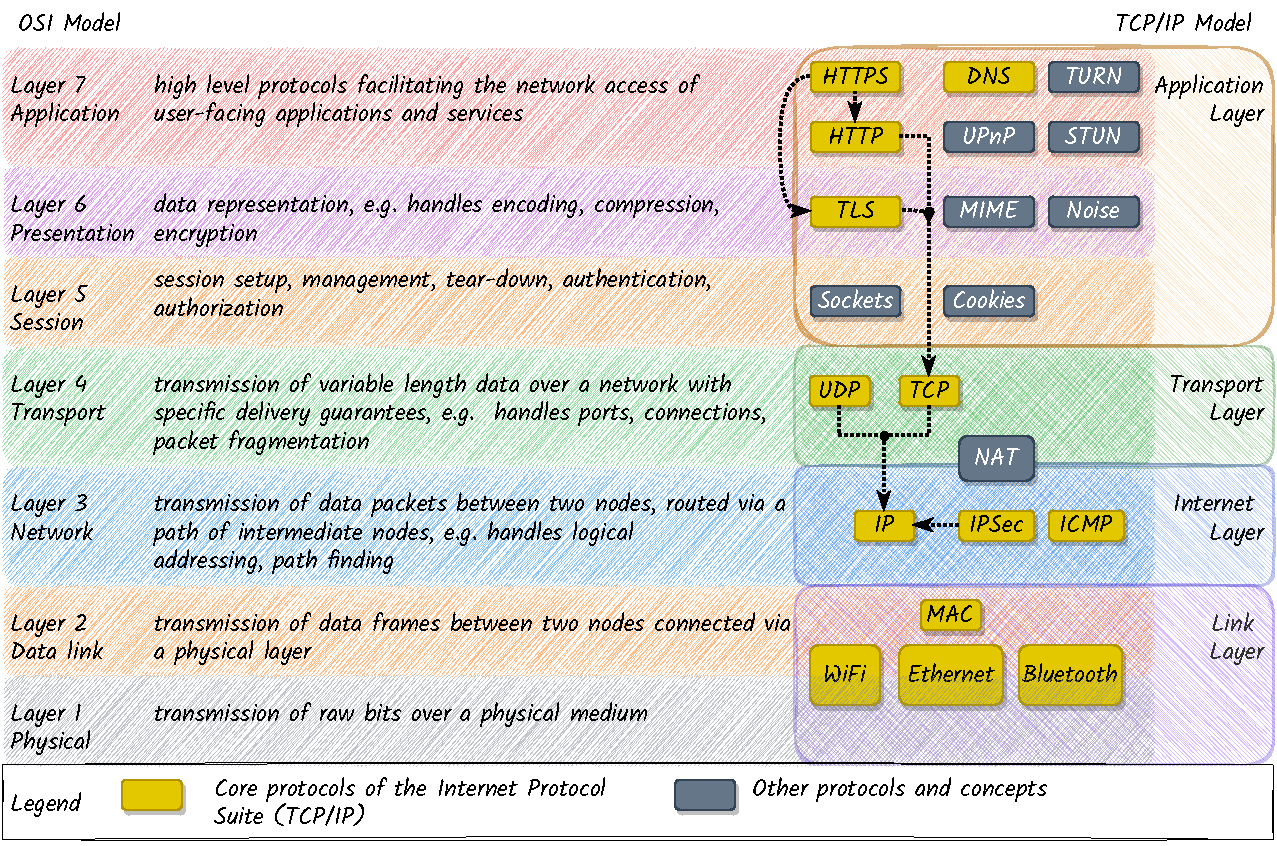
\includegraphics[width=1\textwidth,height=\textheight]{thesis/../figures/osi-map-tcp.drawio.pdf}
\caption{OSI model mapping of the Internet Protocol
Suite\label{osi-map-tcp}}
\end{figure}

Communication protocols are usually organized into abstraction layers
based on the scope of their functionality with higher-layer protocols
relying on the services provided by the lower-layer protocols. Several
reference models define different layering schemes, for example, the OSI
model recognizes 7 layers, while TCP/IP itself combines some of the
layers and recognizes 4. Figure \ref{osi-map-tcp} shows how the two
models relate to each other and describes the responsibilities of the
various layers. Throughout this thesis, we will refer to the 7 layer
numbers of the OSI model as they are more widely used in the literature.

The packets that are transmitted over the network contain information
from multiple protocols organized in \glspl{pdu} with the lower-layer
PDUs \textbf{encapsulating} the higher-layer PDUs as a (usually opaque)
\textbf{payload}. Additionally, the PDU of a protocol contains control
information for the protocol itself in the form of a \textbf{header} or
\textbf{footer}.

Services that are implemented as Application layer (L7) protocols on top
of TCP/IP include the \gls{www}, file transfer (\as{ftp}), email
(\as{smtp}), instant messaging, remote access (\as{ssh}
\autocite{sshRFC}) and others. The Web is a collection of interconnected
documents that use Web technologies such as \as{html} and JavaScript. It
is typically accessed via a user-agent software such as a \textbf{Web
Browser}.

The following sub-sections will briefly cover the main protocols of the
Internet Protocol Suite, the issues for multiparty communications and
some of the low-level mitigation techniques.

\todo{add a paragraph that describes what the rest of the section will contain}

\section{Communication
Protocols}\label{thesis__020-internet.md__communication-protocols}

\subsection{Network Layer
(L3)}\label{thesis__020-internet.md__network-layer-l3}

The \as{ip} \autocite{ipv4RFC} is a Network layer (L3) protocol of the
Internet Protocol Suite that is responsible for transferring datagrams
between devices across the boundaries of their \glspl{lan} by possibly
routing them via multiple intermediate devices (e.g.~routers). A
datagram is a self-contained unit of data, typically associated with
connectionless protocols that provide no guarantees for delivery or
ordering (e.g.~IP, UDP).
\todo{packet is the physical envelope of the IP datagram} IP datagrams
have a header that contains fields such as the \textbf{IP addresses} of
its source and destination, and a
\todo{show a diagram of the internet with multiple local networks}
payload that encapsulates the data from the Transport Layer (L4)
protocols. A \textbf{router} is a device that is part of multiple
networks and relays datagrams between them based on a routing table that
maps IP address ranges to networks.

\subsection{Transport Layer
(L4)}\label{thesis__020-internet.md__transport-layer-l4}

\af{udp} is a very thin Transport layer (L4) protocol that only provides
port multiplexing and checksumming on top of IP. - Port multiplexing -
uses 16-bit numbers to allow multiple processes behind the same IP
address to establish their own communication channels - Checksumming -
used to detect errors in the datagram header and payload

As with IP, UDP packets are referred to as datagrams because they are
not delivered reliably and if such features are required, they must be
implemented by the consumer of the protocol.

\gls{tcp} is another Transport layer (L4) protocol. Like UDP, it
provides port multiplexing and checksumming, but it offers stronger
delivery guarantees. Some of the features it offers are listed below:

\begin{itemize}
\tightlist
\item
  Connection management - TCP establishes reliable connections between
  the communicating hosts and can gracefully terminate them when
  required
\item
  Segmentation - TCP splits variable-length data streams into segments
  that fit inside IP datagrams and transmits them individually
\item
  ordering - segments have sequence numbers to ensure that they are
  reassembled in the correct order at the receiving host
\item
  Error detection and correction - TCP retransmits a segment if its
  checksum fails
\end{itemize}

Both TCP and UDP are useful in different scenarios. UDP is faster and is
used for applications that can tolerate packet loss, e.g.~video
streaming, VoIP, or in cases where it is preferable for an application
to implement its own reliable delivery. TCP has a higher overhead than
UDP but its reliable delivery is a good default for most applications on
the Internet.

\gls{quic} is a more recent Transport layer (L4) protocol that is built
on top of UDP and offers similar features to TCP, but with lower latency
in some scenarios. It provides an additional level of multiplexing
within a process, which allows multiple streams of data to be sent over
the same connection asynchronously. To better optimize the establishment
of secure connections, QUIC is tightly coupled with \as{tls} version
1.3. One of the main uses of QUIC is inside \as{http} version 3.

\subsection{Application Layer
(L7)}\label{thesis__020-internet.md__application-layer-l7}

\gls{http} is an Application layer (L7) protocol that enables stateless
request/response interactions on the Web between web servers and clients
(e.g.~browsers). Similar to other L7 protocols, it uses \glspl{url} for
locating resources.

\begin{description}
\item[URL format:]
\texttt{scheme://host:port/path?query=value\#fragment}
\item[URL example:]
\texttt{http://www.example.com:80/path/to/file.html}.
\end{description}

HTTP up to version 2 uses TCP as a transport protocol and since version
3 uses \as{quic}. HTTP provides several features such as:

\begin{itemize}
\tightlist
\item
  Request Methods - used by the client to specify the action to perform
  on the resource behind the given URL, e.g.~GET, POST, PUT, DELETE,
  etc.
\item
  Headers - used to provide additional information about a request or
  response, e.g.~Content-Type, Authorization, Cache-Control
\item
  Status codes - used to indicate the result of a request, e.g.~if it
  was successful (200), or if the resource is missing (404)
\item
  Cookies - used to include stateful information about the user kept on
  the client-side
\item
  Caching - used to specify that the result of a request can be cached
  for a certain time to avoid repeating the request's action.
\end{itemize}

The \gls{dns} operates at the Application Layer (L7) and allows the
conversion of human-readable domains to IP addresses,
e.g.~\texttt{google.com} to \texttt{142.250.179.142}.

\section{Secure Communication
Protocols}\label{thesis__020-internet.md__secure-communication-protocols}

The communication protocols from the previous section do not encrypt the
payloads of their packets, which allows intruders and routers between
the communicating hosts to see the data. This section provides an
overview of protocols that provide security to those communication
protocols.

\subsection{Transport Layer (L4) to Application Layer
(L7)}\label{thesis__020-internet.md__transport-layer-l4-to-application-layer-l7}

\af{tls} \autocite{tlsRFC} and its precursor \gls{ssl} are protocols
that provide secure communications to Application layer (L7) protocols
on top of a reliable Transport layer (L4) protocol like \gls{tcp}.
\gls{dtls} is a related protocol that works with connectionless
transport protocols like \as{udp}. TLS is usually placed somewhere
between the Presentation layer (L6) and the Transport layer (L4) because
Application layer (L7) protocols use it as a transport protocol while
having to manage the TLS connections.

TLS relies on digital certificates and \gls{pki} to establish trust
between the communicating parties and to prevent man-in-the-middle
attacks. A certificate includes information such as:

\begin{itemize}
\tightlist
\item
  Subject - an identifiable name for the certificate's owner. Depending
  on the use case it can be a domain name, an IP address, an email
  address or others.
\item
  Subject's public key - an asymmetric public key that is used by other
  parties to verify that they are communicating with the subject who is
  expected to be in control of the corresponding private key. The public
  key can also be used to encrypt messages that only the subject can
  decrypt.
\item
  Issuer - an entity that is responsible for validating the identity of
  the subject. It is usually a \gls{ca} that is trusted by the consumer
  of the certificate, but in the case of a self-signed certificate, it
  can be the subject itself
\item
  Issuer's signature - a signature of the certificate's contents using
  the issuer's private key
\end{itemize}

Trusted CAs that serve as the root of trust are usually included in the
operating system or a Web browser. This allows applications to verify
the certificates of the servers they communicate with. Web browsers use
\gls{https} \autocite{httpsRFC} - a variant of \gls{http} that uses TLS
to secure the underlying \as{tcp} or \as{quic} connections of Web
applications. The one-way approach where only the server has to
authenticate itself to the clients is usually sufficient for most web
interactions. TLS can also be used for mutual authentication, where both
of the communicating parties have to present a valid certificate to each
other, but this requires additional infrastructure to manage the
client-side certificates. This mode of operations is sometimes used in
Zero Trust networking, in microservice architectures and TLS-based
\as{vpn} applications.

Due to asymmetric cryptography being computationally expensive, TLS uses
a hybrid approach. The communicating parties use the asymmetric key/s
and Diffie--Hellman key exchange to agree on a set of symmetric session
keys for authentication and encryption/decryption of their data.

TLS is rather complex because it needs to support many possible use
cases while remaining backward compatible. It allows the negotiation of
security parameters like cipher suits.

TLS operates at the Transport layer (L4) and above so it encrypts the
application traffic, but not the IP datagrams. While an \as{isp} or an
intruder with access to the network cannot decrypt the traffic to see
what is being communicated, it could see which IP addresses are
communicating with each other.

\af{ssh} is an Application layer (L7) protocol that allows a client to
securely log in and execute commands on a remote server. It does not
rely on TLS but uses similar cryptographic primitives. Both the client
and the server must authenticate to each other using public-key
cryptography or a password. The cryptographic material must be
distributed via a side channel either manually or via automation tools.

\subsection{Network Layer
(L3)}\label{thesis__020-internet.md__network-layer-l3-1}

Network layer (L3) security protocols provide host-to-host security in
Internet Protocol communications. Their implementations are usually
configured in the operating systems of the hosts and are invisible to
the higher-layer protocols that depend on the Internet Protocol.

\subsubsection{IPSec}\label{thesis__020-internet.md__ipsec}

\af{ipsec} is a Network layer (L3) protocol suite that provides
host-to-host secure communications between \as{ip} hosts. It has two
modes of operation:

\begin{itemize}
\tightlist
\item
  Transport mode - encrypts the payload of an IP datagram, but not the
  header. This mode secures the traffic between two network hosts, but
  similarly to \as{tls}, the routers between the hosts can still see the
  IP addresses of the hosts and the ports they are communicating on
\item
  Tunneling mode - encrypts the entire IP datagram and encapsulates it
  in a new IP datagram with an unencrypted header. This mode is used for
  secure comm allows a host to decrypt the encapsulated both the traffic
  connection between a client and a server that can decrypt the
  encapsulated IP datagram and forward it to its destination.is often
  used to securely connect a client to a server that can decrypt the
  encapsulated IP datagrams and forward them to their destination. The
  client
\end{itemize}

\todo{\as{vpn}  This way the VPN client can hide the IP addresses of the final destinations of the traffic from hosts between itself and the VPN server. Depending on the use case, the VPN server could either facilitate the client's secure access to other resources on the virtual network, or provide anonymity to the VPN client by hiding its IP address from the hosts its communicating with on the public Internet.}

IPSec always requires mutual authentication, unlike \as{tls}, where it
is optional. Authentication can be achieved either via digital
certificates, \glspl{psk} or others.

\todo{The Internet Protocol Security (IPSec) protocol suite is designed specifically to provide secure communication between two hosts at the network layer (L3) of the OSI model. IPSec can be used to secure traffic between two hosts, between a host and a network, or between two networks. It provides a range of services, including data confidentiality, data integrity, and authentication, and is often used in Virtual Private Network (VPN) connections to create secure tunnels between remote networks. IPSec operates in either Transport or Tunnel mode, and can use either the Authentication Header (AH) or Encapsulating Security Payload (ESP) protocols to provide its security services.}

\todo{
- \af{ipsec}
  - Layer 3 protocol suite part of the Internet Protocol Suite
  - used inside VPN software
  - has implementations in both user and kernel space as well as hardware implementations
  - rewrites and encrypts the IP headers and payloads
  - virtual routing table
  - Initially was built into IPv6, separate from IPv4
}

\subsubsection{OpenVPN
Protocol}\label{thesis__020-internet.md__openvpn-protocol}

\begin{itemize}
\tightlist
\item
\item
\item
\item
\end{itemize}

\subsubsection{WireGuard}\label{thesis__020-internet.md__wireguard}

WireGuard \autocite{donenfeldWireGuardNextGeneration2017} is a more
recent protocol with a design informed by lessons learned from IPSec and
OpenVPN and a key management approach inspired by \as{ssh}. It is a
lower-level protocol that focuses on configuration simplicity while
network topology, peer discovery and key distribution are left as a
responsibility of higher-level systems that use it as a building block.
Wireguard is implemented as a Layer 3 overlay over UDP tunnels.
WireGuard has both user-space implementations that use a TUN driver and
also has direct support built into the Linux Kernel since version 5.6
(May 2020). The kernel implementation allows for better performance
because it does not need to copy packets between the kernel and
user-space memory.

WireGuard's cryptography is based on the \textbf{Noise Protocol
Framework}\autocite{noiseDocs}. Noise is another recent effort that
applies the ideas of TLS in a simplified way. It serves as a blueprint
for designing use-case-specific protocols for establishing secure
communication channels based on \gls{ecdh} handshake patterns. It powers
the end-to-end encryption in messaging applications such as WhatsApp and
Signal, and \gls{vpn} software such as WireGuard and Nebula.
\todo{elaborate} \todo{noise is transport agnostic}
\todo{noise has limited cipher suites}

The snippets below show a minimal set of configuration options that need
to be provided for two peers to be able to form secure tunnels with each
other.

\begin{Shaded}
\begin{Highlighting}[]
\CommentTok{\# peer1.conf}
\KeywordTok{[Interface]}
\DataTypeTok{Address }\OtherTok{=}\StringTok{ 101.0.0.1/32}
\DataTypeTok{ListenPort }\OtherTok{=}\StringTok{ }\DecValTok{53063}
\DataTypeTok{PrivateKey }\OtherTok{=}\StringTok{ ePTiXXhHjvAHdWUr8Bimk30n0gh3m241RAzsN0JZDW0=}

\KeywordTok{[Peer]}
\DataTypeTok{PublicKey }\OtherTok{=}\StringTok{ BSn0ejd1Y3bKuD+Xpg0ZZeOf+Ies/oql0NZxw+SOmkc=}
\DataTypeTok{AllowedIPs }\OtherTok{=}\StringTok{ 101.0.0.2/32}
\DataTypeTok{Endpoint }\OtherTok{=}\StringTok{ peer1.example.com:38133}
\end{Highlighting}
\end{Shaded}

\begin{Shaded}
\begin{Highlighting}[]
\CommentTok{\# peer2.conf}
\KeywordTok{[Interface]}
\DataTypeTok{Address }\OtherTok{=}\StringTok{ 101.0.0.2/32}
\DataTypeTok{ListenPort }\OtherTok{=}\StringTok{ }\DecValTok{38133}
\DataTypeTok{PrivateKey }\OtherTok{=}\StringTok{ sN/d6XUPEVPGSziVgCCOnOivDK+qAoYC3nxnssQ5Rls=}

\KeywordTok{[Peer]}
\DataTypeTok{PublicKey }\OtherTok{=}\StringTok{ e/TxvPmrgcc1G4cSH2bHv5J0PRHXKjYxTFoU8r+G93E=}
\DataTypeTok{AllowedIPs }\OtherTok{=}\StringTok{ 101.0.0.1/32}
\end{Highlighting}
\end{Shaded}

Each peer has a public/private key pair that is used for authentication
and encryption based on the Noise Protocol Framework
\autocite{noiseDocs}. The \texttt{Address} field specifies the virtual
IP address that the local network interface will use, while the
\texttt{AllowedIPs} field specifies what virtual IP addresses are
associated with a peer's public key. A peer's \texttt{Endpoint} field
specifies the URL at which it can be reached. Only one of the peers must
be configured with a reachable endpoint for the other one. In the above
example once \texttt{peer1} initiates communication with \texttt{peer2},
\texttt{peer2} will learn the current endpoint of \texttt{peer1} and
will be able to communicate back with it.

\todo{ \gls{cidr} is a common notation for describing IP address ranges, e.g. `192.168.0.1/16`, where the number after the slash describes the bit-length of the fixed prefix for a subnet.}

\section{Challenges and Solutions for Multiparty
Communications}\label{thesis__020-internet.md__challenges-and-solutions-for-multiparty-communications}

The version of the Internet Protocol, that was originally deployed
globally (IPv4), uses 32-bit numbers as IP addresses, allowing for
around 4 billion unique addresses. Due to the popularity of the
Internet, there are many more devices than available IPv4 addresses,
which has caused challenges. IPv6 is a newer version of the protocol
that uses a larger 128-bit address space which is sufficient for
assigning 100 addresses for each atom on Earth. However, its adoption
has been slow, as according to Google\autocite{IPv6Google} as of 2023
around 41\% of their users access their services over IPv6.
Additionally, despite that IPv6 allows for all devices to be addressable
on the Internet, for security reasons, most of them would use firewalls
to block incoming remote traffic that is not associated with outgoing
connections.

A widespread solution to the addressing problem is \gls{nat}. It allows
many devices without globally unique IP addresses to initiate
connections to publicly addressable devices on the Internet via a
limited number of gateways that must have globally unique IP addresses.
A NAT gateway replaces the local source IP address of each outgoing IP
datagram with its own public IP address before passing it on to the next
link on the way to the destination while maintaining a mapping between
the source and destination IPs in a translation table. The destination
host can then address its responses back to the NAT gateway's public IP
address, which in turn replaces its own IP from the incoming datagrams
with the IP of the local device and forwards them to it. If the IP
datagrams encapsulate TCP/UDP packets, the gateway additionally rewrites
the source and destination ports, which means that NAT techniques can be
placed somewhere between Layers 3 and 4 of the OSI model.

The effect of NAT on connectivity is similar to an IPv6 firewall as they
both allow devices on a local network to initiate bidirectional
communication to remote devices with public IP addresses, but
connections cannot be natively initiated by the remote devices. As
Figure \ref{nat-intro} shows, it follows that when two devices are
behind separate NATs, neither can contact the other first.
\textbf{Client/Server} communication is less affected by this limitation
because Servers are usually deployed to a public IP address that can be
contacted by Clients with local IP addresses. \textbf{Peer-to-Peer}
communication, however, is more challenging because the peers are often
devices in separate residential networks behind different NATs. Several
\textbf{NAT traversal} techniques try to solve this with different
performance tradeoffs and success that varies depending on the NAT
\autocite{natBehaviorRFC} and its behavior when mapping ports and IP
addresses.
\todo{describe some of the nat behaviors, e.g. if the source IP address/port vary per destination are changed depending on the destination/port mapping algorithms, if it maps ports, IPs, whether the mapped IPs are different per destination and others.}

\begin{figure}
\centering
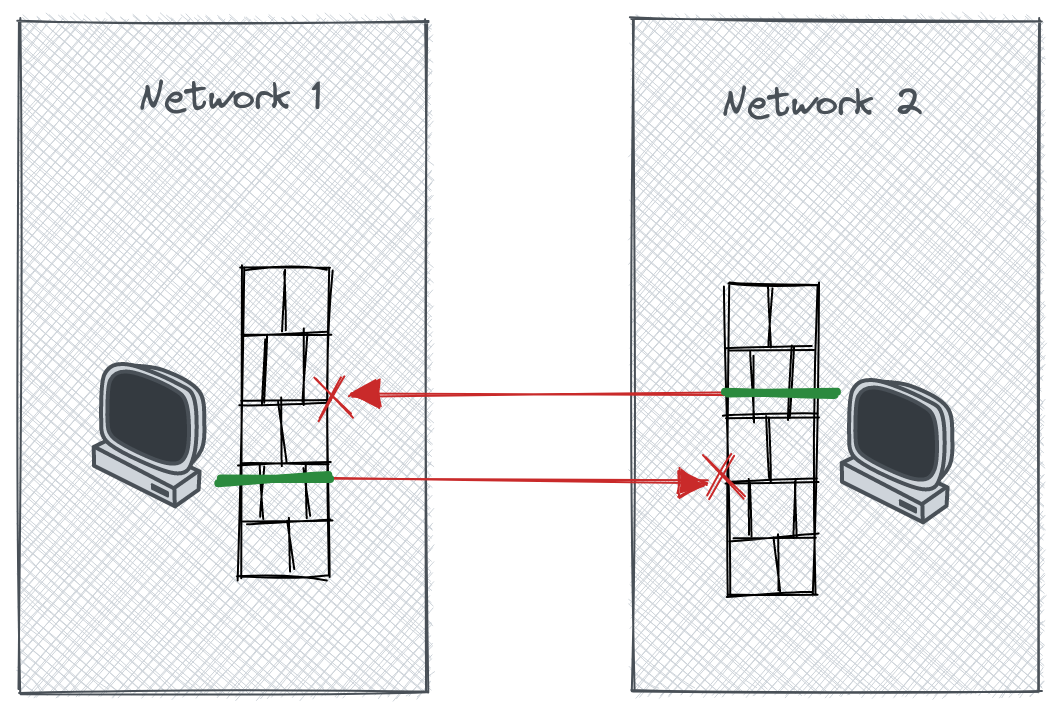
\includegraphics[width=\textwidth,height=0.25\textheight]{thesis/../figures/nat-intro.png}
\caption{Two parties behind separate NATs\label{nat-intro}}
\end{figure}

One approach based on the Client/Server model is to use a publicly
addressable \textbf{relay} server that is contacted by the NATed devices
and then forwards the Peer-to-Peer traffic to the intended recipient.
Compared to direct communication, relaying results in a higher network
latency due to the longer path that each packet must travel. Maintaining
a relay server requires some technical expertise and may be costly
depending on the expected throughput. Despite the drawbacks, relaying
works under most networking scenarios and is therefore often used as a
fallback in case all other approaches fail to find a direct path.
Protocols such as \af{turn} \autocite{turnRFC} and \af{derp}
\autocite{derpDocs} can be used to securely implement relaying.

The NAT gateway in many residential networks is a Router device under
the customer's control that has a statically or dynamically assigned
public IP address. Most routers can be manually configured through their
admin page to forward all traffic that arrives at a given port to a
specific device on the local network. Remote applications can then
initiate a connection to the local device if they know the IP address of
the router and the forwarded port. The manual configuration, however,
can be inconvenient and many users may be unaware of that setting
because it is not necessary for the more straightforward Client/Server
communications. Some routers also support programmatic configuration of
port forwarding via a Layer 7 protocol like \gls{upnp} or its successors
\gls{nat-pmp} and \gls{pcp}. However, these protocols are not always
supported and are often disabled by the local network administrators due
to security concerns related to bugs in their implementation, vulnerable
IOT devices on the local network or malicious programs being able to
expose local devices to the internet.

\todo{connection reversal}

An efficient NAT traversal approach that works with some types of NATs
is to use \gls{stun} \autocite{stunRFC} in combination with \as{udp}
hole punching (Figure \ref{nat-traversal}). STUN is a protocol operating
at Layer 7 that allows a client application to detect the presence of
NAT gateways on the network path to a public STUN server, and identify
their types and the public IP address that they map to externally. The
process usually involves the following steps:

\begin{itemize}
\tightlist
\item
  An application sends \as{udp} datagrams to the STUN server (1, 3 in
  fig.~\ref{nat-traversal})
\item
  The STUN server responds with the source IP address and port specified
  inside the datagrams (2, 4 in fig.~\ref{nat-traversal})
\item
  The application compares its own endpoint with the source endpoint
  observed by the STUN server and if the values differ, it can be
  inferred that they were rewritten by a NAT. Additional STUN servers
  are contacted to determine if the NAT maps IPs and ports in a
  predictable fashion.
\end{itemize}

UDP hole punching is a related technique that, depending on the NAT
types, can allow direct communication between two applications behind
separate NATs. The applications must discover each other's externally
mapped endpoints, perhaps via the STUN server. \todo{If, else?} If the
NATs use the same external port regardless of the remote destination:

\begin{itemize}
\tightlist
\item
  The two applications simultaneously send UDP packets to each other's
  external endpoints (5 in fig.~\ref{nat-traversal})
\item
  Their respective NATs will process the outgoing packets to the other
  peer and create a port mapping for the reverse traffic - a ``punched
  hole''
\item
  When the incoming traffic from a peer arrives at the other peer's NAT,
  it will be forwarded correctly due to the port mapping that was
  created earlier
\end{itemize}

NATs that map different ports per remote destination sometimes allocate
port numbers predictably, which can be used by the peers to try to guess
the port that will be opened by the opposing side's NAT.

\todo{Talk about traversal friendly NATs and unfriendly NATs}
\todo{add a bullet list with the steps in the STUN process and relate them to the step numbers in the figure}

\begin{figure}
\centering
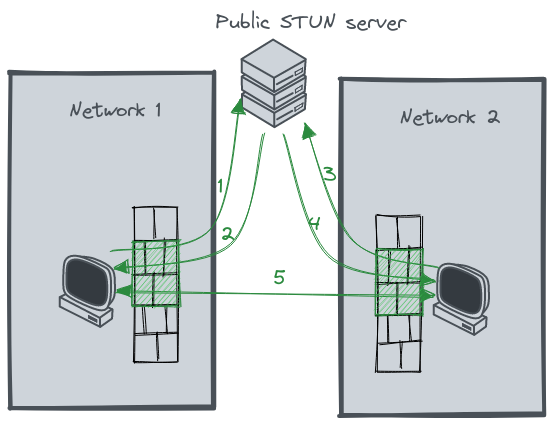
\includegraphics[width=\textwidth,height=0.25\textheight]{thesis/../figures/nat-traversal.png}
\caption{NAT traversal via STUN\label{nat-traversal}}
\end{figure}

In mobile networks like 4G and 5G, the \gls{isp} often utilizes a
\gls{cgnat} as part of their infrastructure, while all devices under the
user's control, including the router, only have local IP addresses. STUN
techniques would fail to discover a direct path between two parties
behind separate CGNATs or other unpredictable NAT algorithms. The only
remaining possibility is to relay the traffic via a publicly reachable
third-party host using a protocol similar to TURN.
\todo{only ~65000 ports per IP address means that CGNATs that provide more than 65000 connections from client devices require more than one public IP address}

\todo{hairpinning - Hairpinning, also known as NAT loopback or NAT reflection, is a technique used by NAT devices to allow hosts on a private network to access a public server using its public IP address. Without hairpinning, the NAT device would not recognize the connection as a loopback connection and would route it to the public network, causing the connection to fail. With hairpinning, the NAT device recognizes that the connection is a loopback connection and redirects the traffic back to the same NAT device, which then forwards the traffic to the correct host on the private network. This can be useful in scenarios where a private network is hosting a public-facing server that is also accessed by internal users on the same network using its public IP address.}

\gls{ice} is a protocol that describes a standard way for peers to
gather candidate addresses for direct communication via STUN and TURN
and then exchange them via a signaling server. The protocol continuously
checks which candidates provide the best connection and adjusts them.

\gls{webrtc} is a framework that allows peer-to-peer communications
between Web applications in Web browsers. Web applications are normally
limited to HTTP connections and cannot use raw UDP or TCP connections.
WebRTC implements the ICE functionality in Web browsers and provides an
API to Web applications.

\todo[caption={webrtc}]{
- ICE

- encryption

- Reveals IP addresses
}

\phantomsection\label{thesis__022-overlays.md}
\chapter{Overlay Networks}\label{thesis__022-overlays.md__sec:overlays}

An \textbf{overlay network} is a higher-order solution that provides
additional networking functionality on top of an existing underlay
network like the Internet. From the point of view of its consumers, an
overlay network may appear at a lower OSI layer, despite being
implemented using protocols from higher layers. For example \glspl{vpn}
can provide virtual interfaces to the Operating System at the Link layer
(L2) or Network layer (L3) while being implemented on top of a Transport
layer (L4) protocol like \gls{udp} or a Presentation layer (L6) protocol
like \gls{tls}. Virtual IP addresses can be assigned to the hosts and
applications that are already designed to work with TCP/IP can directly
use the virtual network interfaces via the regular TCP/IP mechanisms
provided by the operating system.

Other overlay networks are both implemented and used at the Application
layer (L7). To communicate via such an overlay network, applications
often have to implement specific functionality in their software by
utilizing a framework or a library.

Figure \ref{osi-map-overlays} shows an approximate OSI model mapping of
several protocols and network overlay solutions from the point of view
of the systems that use them and the arrows show dependency relations
between them.

\begin{figure}
\centering
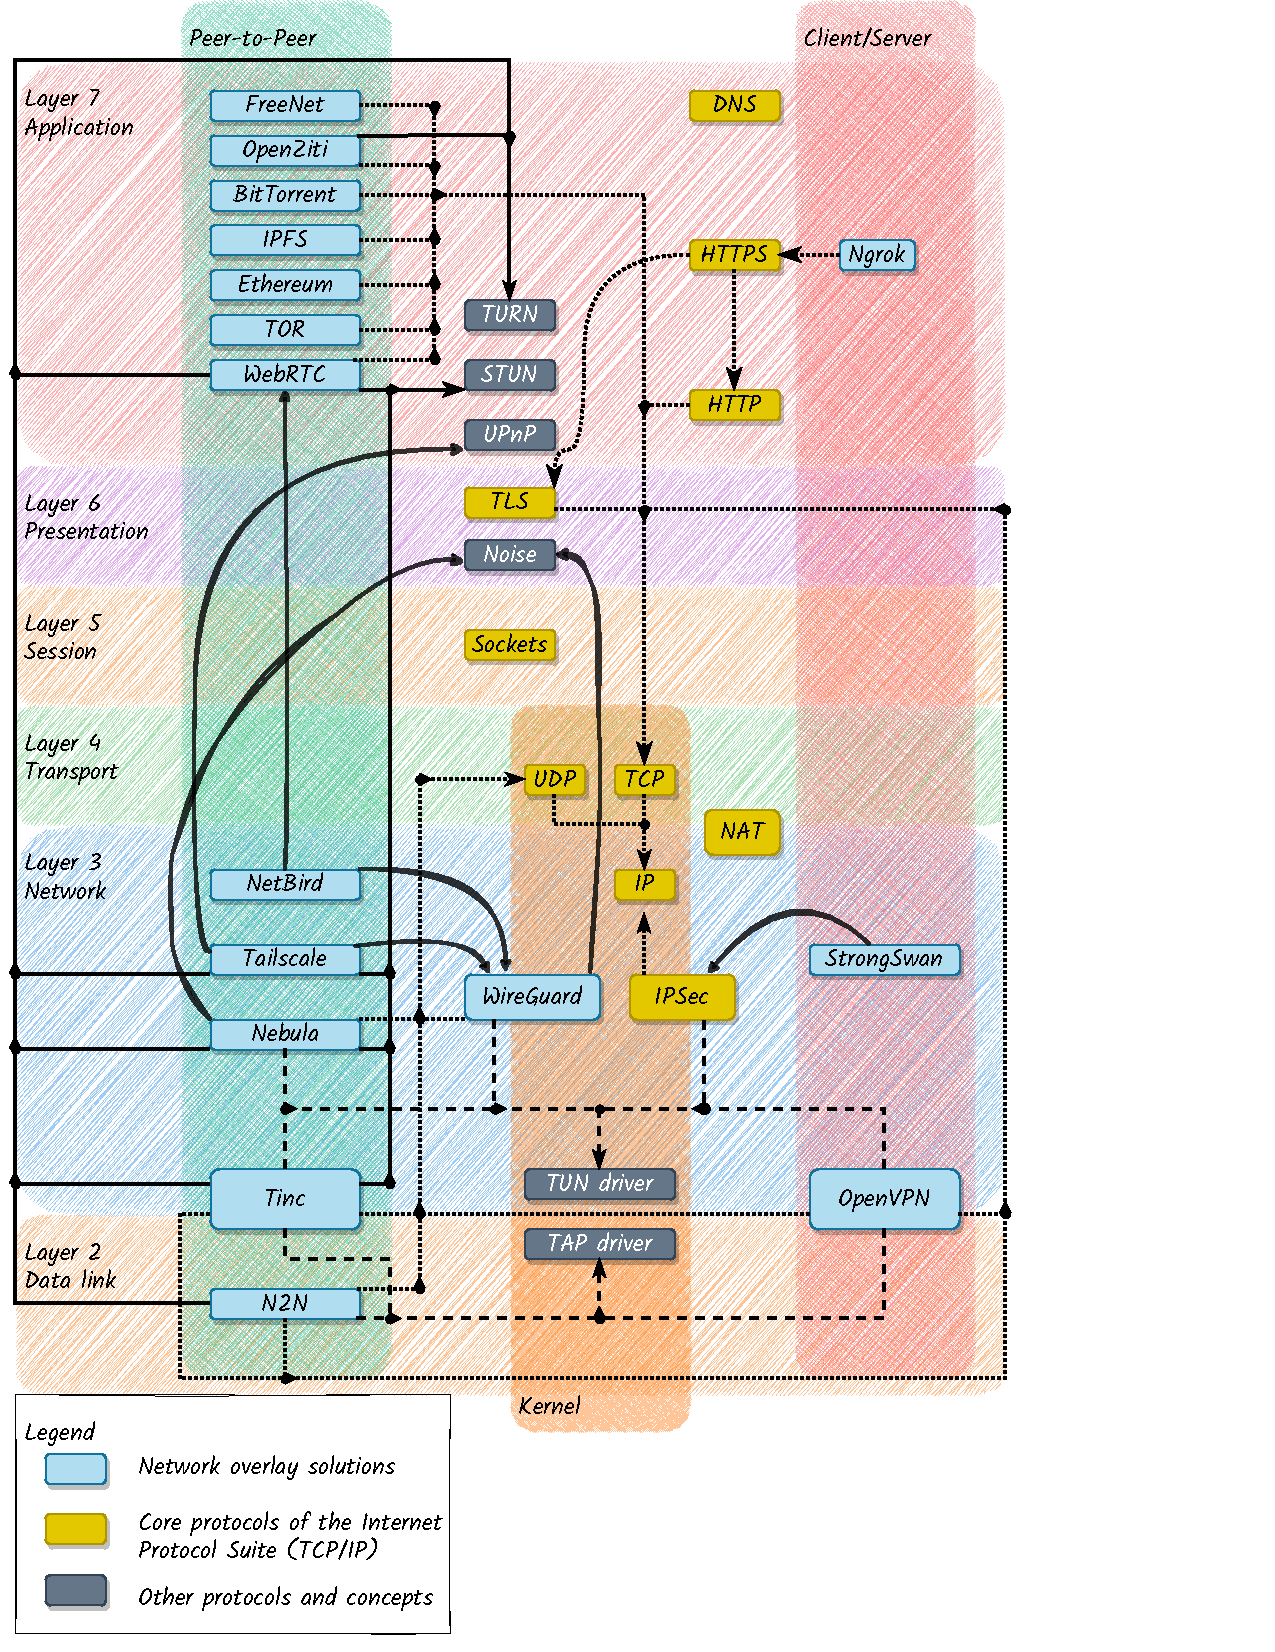
\includegraphics[width=\textwidth,height=0.9\textheight]{thesis/../figures/osi-map-overlays.drawio.pdf}
\caption{OSI model mapping of various protocols
\label{osi-map-overlays}}
\end{figure}

\section{Data Link Layer (L2) and Network Layer
(L3)}\label{thesis__022-overlays.md__data-link-layer-l2-and-network-layer-l3}

\subsection{Client/Server
VPNs}\label{thesis__022-overlays.md__clientserver-vpns}

Layer 2 virtual networks provide a virtual network switch that allows
remote machines to be on the same virtual LAN and share the same IP
address range. Layer 3 virtual networks provide a virtual network router
that allows remote machines to be on separate LANs. Depending on the
specific implementation, the overlay network can either be implemented
directly in the Operating System's kernel, or on top of a driver like
\as{tun} or \as{tap}.

\begin{itemize}
\tightlist
\item
  Layer 2 vs Layer 3 Networks

  \begin{itemize}
  \tightlist
  \item
    Layer 2 overlay networks bridge other networks

    \begin{itemize}
    \tightlist
    \item
      virtual network switch
    \item
      remote machines are on the same virtual LAN and can share the same
      IP address range
    \item
      allows broadcast/multicast
    \item
      TAP driver
    \end{itemize}
  \item
    Layer 3 overlays route traffic between separate local networks

    \begin{itemize}
    \item
      virtual network router
    \item
      remote machines are on separate LANs
    \item
      simpler to configure
    \item
      TUN driver
    \item
      the low-level solutions from the previous section are complex to
      set up.
    \item
      overlay networks package some of those solutions for a specific
      use case Most overlay networks use a combination of the NAT
      traversal techniques mentioned previously. They can be placed in
      Layers 2, 3 or 7. Layer 2 overlays act as a virtual network
      switch, while Layer 3 overlays act as a virtual network router.
      Layer 7 overlays are implemented in user-space as libraries or
      applications that run on top of the network stack of the host
      operating system. Layer 2 and 3 overlays can either be implemented
      as kernel modules or as user-space applications that use a
      \textbf{TUN/TAP} \todo{explain the names} driver to interface with
      the kernel.
    \end{itemize}

    \todo{tls vs ipsec vpns. TLS vpns offer a virtual network interface at layer 3, but run over L7 TLS }

    \begin{itemize}
    \tightlist
    \item
      The term ``VPN'' is somewhat overloaded as it can refer to
      different related concepts.
    \end{itemize}

    \glspl{vpn} are implemented as Layer 2 or 3 network overlays. They
    are commonly used for securely connecting machines from different
    \glspl{lan}. They provide software emulation of a network interface
    controller via a TUN/TAP driver on the operating system level and
    allow other software to transparently use the functionality of the
    \gls{ip} suite without requiring extra changes. Traditional
    \glspl{vpn} such as IPSec \autocite{ipSecRFC} and OpenVPN
    \autocite{openVPNDocs} use a centralized service that all
    (encrypted) client communications must pass through. This introduces
    a single point of failure and a potential bottleneck that might
    negatively impact the performance of the multiparty computations due
    to their \gls{p2p} nature.
  \end{itemize}
\end{itemize}

\subsubsection{OpenVPN
Client/Server}\label{thesis__022-overlays.md__openvpn-clientserver}

We already discussed the VPN protocol behind OpenVPN. Here we will go
into the client and server software and how they are implemented and
discuss the typical network topologies.

\subsection{Mesh VPNs}\label{thesis__022-overlays.md__mesh-vpns}

\begin{itemize}
\tightlist
\item
  Tinc
\item
  N2N
\item
  Tailscale
\item
  Nebula
\item
  ZeroTier
\end{itemize}

Mesh \glspl{vpn} such as Tinc \autocite{tincDocs}, Tailscale
\autocite{tailscaleDocs} and Nebula \autocite{nebulaDocs} utilize NAT
Traversal techniques to create direct \gls{p2p} links between the
clients for the data traffic. Authentication, authorization and traffic
encryption are performed using certificates based on public key
cryptography.

All three are open-source, except Tailscale's coordination service which
handles peer discovery and identity management. Headscale
\autocite{fontJuanfontHeadscale2022} is a community-driven open-source
alternative for that component. Tinc is the oldest of the three but has
a relatively small community. It is mainly developed by a single author
and appears to be more academic than industry motivated. Nebula and
Tailscale are both business driven. Tailscale was started by some
high-profile ex-googlers and is the most end-user-focused of the three,
providing a service that allows people to sign up using identity
providers such as Google, Microsoft, GitHub and others. They also
provide an Admin console that allows a user to easily add their personal
devices to a network or share them with others. It also has support for
automation tools like Terraform for creating authorization keys and
managing an \gls{acl} based firewall. Nebula was originally developed at
the instant messaging company Slack to create overlay networks for their
cross-region cloud infrastructure, but the authors later started a new
company and are currently developing a user-centric platform similar to
Tailscale's. Nebula is more customizable than Tailscale and since it is
completely open-source it can be adapted to different use cases, but it
is also more involved to set up. A certificate authority needs to be
configured for issuing the identities of the participating hosts.
Furthermore, publicly accessible coordination servers need to be
deployed to facilitate the host discovery. Tailscale employs a
distributed relay network of \gls{derp} servers, while Nebula can be
configured to route via one of the other peers in the VPN.

\section{Application Layer
(L7)}\label{thesis__022-overlays.md__application-layer-l7}

\subsection{OpenZiti}\label{thesis__022-overlays.md__openziti}

OpenZiti is a commercial product that provides an SDK for creating
\gls{p2p} overlay networks. It is developed by NetFoundry, a company
that provides a Software as a Service platform for creating and managing
\gls{p2p} overlay networks. The SDK is open-source and can be used to
create custom overlay networks. The SDK is written in Go and provides a
high-level \gls{api} for creating and managing the overlay network. It
uses a centralized service for peer discovery and identity management.
The data traffic is routed via a \gls{p2p} network of relays. The relays
are hosted by NetFoundry and are not open-source. The SDK is available
for Go, Java, Python, C\# and C++.

\todo{edit}

\begin{itemize}
\tightlist
\item
  uses relays
\end{itemize}

\subsection{LibP2P}\label{thesis__022-overlays.md__libp2p}

\begin{itemize}
\tightlist
\item
  libP2P
\item
  ngrok
\item
  TOR
\item
  BitTorrent
\item
  IPFS
\item
  Ethereum
\item
  Teleport
\item
  Freenet
\end{itemize}

\phantomsection\label{thesis__025-identity.md}
\chapter{Digital Identities for Multiparty
Computations}\label{thesis__025-identity.md__digital-identities-for-multiparty-computations}

Digital identity mechanisms provide standardized ways for referring to
entities in the context of digital interactions. We have already seen
some examples of digital identities in the previous chapter:

\begin{itemize}
\tightlist
\item
  \as{mac} addresses - host identities at the Data link layer (L2)
\item
  \as{ip} addresses - host identities at the Network layer (L3)
\item
  Digital Certificates - identities that can be cryptographically
  verified
\end{itemize}

Key concepts related to digital identity mechanisms include:

\begin{itemize}
\tightlist
\item
  Issuance - the process of assigning a digital identity to an entity.
  Often this involves a trusted third party like a government or a
  digital identity provider like Google or GitHub. Another option is
  \as{ssi} where a user manages their own identity.
\item
  Authentication - the process of verifying the identity of an entity
\item
  Credentials - use case-specific attributes associated with an identity
\item
  Authorization - the process of verifying if an identity's owner is
  allowed to perform an action on a resource
\end{itemize}

Other notable examples include:

\begin{itemize}
\tightlist
\item
  Email addresses - identities for entities participating in email
  communications
\item
  User names - user identities in various digital platforms that can be
  verified via a password
\item
  ID cards - government-issued identity documents are increasingly able
  to support digital interactions
\item
  Biometrics - used to prove an identity via sensor data
\end{itemize}

\begin{itemize}
\tightlist
\item
  IP addresses

  \begin{itemize}
  \tightlist
  \item
    Cryptographically Generated Addresses - rfc3972
  \item
    Privacy Extensions - rfc4941
  \item
    DNS
  \end{itemize}
\item
  MAC addresses
\item
  Government

  \begin{itemize}
  \tightlist
  \item
    ID Cards / Passports

    \begin{itemize}
    \tightlist
    \item
      NFC
    \end{itemize}
  \item
    Estonia's Digital Government
  \item
    DigiD in NL
  \item
  \end{itemize}
\item
  Certificates
\item
  TLS
\item
  IPSec
\item
  WireGuard
\item
  OpenID Connect
\item
  Crypto currency addresses

  \begin{itemize}
  \tightlist
  \item
    Hierarchical Deterministic Keys
  \item
    ENS
  \end{itemize}
\item
  Self-Sovereign Identity

  \begin{itemize}
  \tightlist
  \item
    Decentralized Identifiers
  \item
    Verifiable Credentials
  \item
    Identity Overlay Network (ION) from Microsoft

    \begin{itemize}
    \tightlist
    \item
      DPKI
    \end{itemize}
  \end{itemize}
\item
  Social Networks

  \begin{itemize}
  \tightlist
  \item
    Centralized

    \begin{itemize}
    \tightlist
    \item
      Facebook
    \item
      Twitter
    \item
      Reddit
    \end{itemize}
  \item
    Decentralized

    \begin{itemize}
    \tightlist
    \item
      Mastodon - Mastodon is an open-source, decentralized social
      networking platform that provides an alternative to traditional
      social media giants like Twitter. It operates on a federated
      model, which means that instead of being a single, centralized
      platform, it is a network of independently operated servers, known
      as ``instances''. Each instance hosts its own community with its
      own rules, but users on any instance can interact with users on
      other instances thanks to a common protocol, creating a connected,
      distributed social network.
    \item
      Bluesky - An ex-twitter initiative to move away from centralized
      social media platforms, where a single organization controls the
      network. Instead, Bluesky aims to develop a standard protocol for
      social media that would enable the development of a variety of
      interoperable, decentralized platforms.
    \item
      Nostr
    \end{itemize}
  \end{itemize}
\item
  Identity Privacy
\end{itemize}

\phantomsection\label{thesis__030-methods.md}
\part{Proof of Concepts and
Evaluation}\label{thesis__030-methods.md__proof-of-concepts-and-evaluation}

\chapter{Testing
methodology}\label{thesis__030-methods.md__testing-methodology}

In the following chapters, we will design and implement several
solutions for ad hoc MPC sessions based on a subset of the previously
discussed related works:

\begin{itemize}
\tightlist
\item
  Internet protocol
\item
  Wireguard
\item
  Tailscale
\item
  Headscale
\item
  ? Headscale with DID identity?
\item
  ? WebRTC?
\item
  A custom solution that automates the WireGuard configuration by
  visiting a web page
\end{itemize}

Additionally, we will analyze and compare them in terms of performance,
security and usability

\section{Measuring
performance}\label{thesis__030-methods.md__measuring-performance}

During the preparation phase of the project, we developed the \gls{e3}
framework which simplifies and automates the process of deploying
machines in different geographical regions, connecting them via an
overlay network and executing multiparty computations between them,
where each machine represents a different party.

To summarize, \gls{e3} is a set of scripts that use several automation
tools:

\begin{itemize}
\tightlist
\item
  Terraform - declarative provisioning
\item
  NixOS - declarative Linux distribution
\item
  Colmena - declarative deployment for NixOS
\item
  PSSH - parallel execution of remote scripts over ssh
\item
  DigitalOcean - a cloud provider
\end{itemize}

It allows us to quickly provision cloud virtual machines in multiple
regions and reproducibly deploy all necessary software for running a
multiparty computation over a chosen network overlay solution. The
source code of \gls{e3} can be found on
\href{https://github.com/e-nikolov/mpyc}{GitHub}

Each solution will be deployed using the \gls{e3} framework and the
performance will be quantitatively measured in terms of the time it
takes to execute several MPyC demos. The selected demos have different
complexities in terms of communication rounds and message sizes which
will allow us to observe their impact on the overall performance.

\begin{enumerate}
\def\labelenumi{\arabic{enumi}.}
\tightlist
\item
  Secret Santa - high round complexity with small messages
\item
  Convolutional Neural Network (CNN) MNIST classifier - low round
  complexity with large messages
\end{enumerate}

The demos will be configured at three different input size levels

\begin{itemize}
\tightlist
\item
  Low,
\item
  Medium
\item
  High
\end{itemize}

Furthermore, the demos will be executed in several networking scenarios:

\begin{enumerate}
\def\labelenumi{\arabic{enumi}.}
\tightlist
\item
  1-10 parties in the same geographic region
\item
  1-10 parties evenly distributed across two nearby regions
\item
  1-10 parties evenly distributed across two distant regions
\item
  1-10 parties distributed across multiple distant regions
\end{enumerate}

\section{Security}\label{thesis__030-methods.md__security}

We will analyze aspects such as

\begin{itemize}
\tightlist
\item
  key distribution
\item
  trust model - are there any trusted third parties and what would be
  the consequences if they are corrupted or breached
\item
  traffic encryption
\item
  identity strength
\end{itemize}

\section{Usability}\label{thesis__030-methods.md__usability}

For each solution, we will describe the steps that the parties need to
perform to execute a joint multiparty computation. Those steps will be
analyzed in terms of:

\begin{itemize}
\tightlist
\item
  Complexity - how much technical expertise is expected from the parties
  to be able to execute the steps
\item
  Initial effort - how much effort is each party expected to put in
  preparing for their first joint computation
\item
  Repeated effort - after the initial setup, how much effort is required
  to perform another computation

  \begin{itemize}
  \tightlist
  \item
    with the same set of parties
  \item
    with another set of parties
  \end{itemize}
\item
  Finalization effort - how much effort is required to finalize the MPC
  session once it is complete and clean up any left-over artifacts or
  resources so that the machine of each party is in its original state
\end{itemize}

\phantomsection\label{thesis__050-internet-protocol.md}
\chapter{Internet Protocol based
solution}\label{thesis__050-internet-protocol.md__internet-protocol-based-solution}

This solution focuses on directly using the internet protocol without
involving an overlay network. Our goal is to analyze the implications of
using only the functionalities that MPyC directly supports to serve as
the reference for our later experiments.

\section{Implementation
details}\label{thesis__050-internet-protocol.md__implementation-details}

We will manually set up the multiparty computations via the public IP
addresses of the machines and DNS.

\section{Performance
analysis}\label{thesis__050-internet-protocol.md__performance-analysis}

\section{Security
analysis}\label{thesis__050-internet-protocol.md__security-analysis}

\section{Usability
analysis}\label{thesis__050-internet-protocol.md__usability-analysis}

\phantomsection\label{thesis__060-wireguard.md}
\chapter{WireGuard based
solution}\label{thesis__060-wireguard.md__wireguard-based-solution}

This solution creates an overlay network by manually configuring
WireGuard on each machine.

\section{Implementation
details}\label{thesis__060-wireguard.md__implementation-details}

\section{Performance
analysis}\label{thesis__060-wireguard.md__performance-analysis}

\section{Security
analysis}\label{thesis__060-wireguard.md__security-analysis}

\section{Usability
analysis}\label{thesis__060-wireguard.md__usability-analysis}

\phantomsection\label{thesis__070-tailscale.md}
\chapter{Tailscale based
solution}\label{thesis__070-tailscale.md__tailscale-based-solution}

Tailscale is a VPN solution that configures a mesh of direct Wireguard
tunnels between the peers.

\section{Implementation
details}\label{thesis__070-tailscale.md__implementation-details}

\section{Performance
analysis}\label{thesis__070-tailscale.md__performance-analysis}

\section{Security
analysis}\label{thesis__070-tailscale.md__security-analysis}

\subsection{Trust model}\label{thesis__070-tailscale.md__trust-model}

There is a centralized service that deals with the key distribution,
which needs to be trusted to provide the correct public keys for the
correct parties

\subsection{Identity}\label{thesis__070-tailscale.md__identity}

Identity is based on third party identity providers such as Microsoft
and GitHub

\begin{itemize}
\item
  Magic DNS
\item ~
  \section{Usability
  analysis}\label{thesis__070-tailscale.md__usability-analysis}
\end{itemize}

With tailscale each party needs to

\begin{itemize}
\tightlist
\item
  register a Tailscale account
\item
  Download and install tailscale on the machine they want to run a
  multiparty computation
\item
  Run tailscale on their machine and logs into their account in order to
  link it to their own Tailnet
\item
  Share their Tailscale machine with the Tailnets of each of the other
  parties
\item
  Download the demo they want to run
\item
  Form the flags for running the chosen demo

  \begin{itemize}
  \tightlist
  \item
    add -P \$HOST:\$PORT for each party using their Tailscale
    hostname/virtual IP
  \end{itemize}
\item
  Run the demo
\end{itemize}

\phantomsection\label{thesis__080-headscale.md}
\chapter{Headscale based
solution}\label{thesis__080-headscale.md__headscale-based-solution}

This solution is similar to the Tailscale one, but it uses Headscale - a
self-hosted open-source alternative to the closed-source Tailscale
coordination service.

\section{Implementation
details}\label{thesis__080-headscale.md__implementation-details}

\section{Performance
analysis}\label{thesis__080-headscale.md__performance-analysis}

\section{Security
analysis}\label{thesis__080-headscale.md__security-analysis}

\subsection{Trust model}\label{thesis__080-headscale.md__trust-model}

There still is a centralized service like in the Tailscale solution, but
here it is self-deployed.

\subsection{Identity}\label{thesis__080-headscale.md__identity}

\section{Usability
analysis}\label{thesis__080-headscale.md__usability-analysis}

\phantomsection\label{thesis__090-mpyc-web.md}
\chapter{MPyC Web}\label{thesis__090-mpyc-web.md__mpyc-web}

This chapter presents the design of MPyC Web - an MPC connectivity
solution based on web technologies (L7) that can run in web browsers.

Design goals:

\begin{itemize}
\tightlist
\item
  Uses the MPyC Python framework
\item
  Runs in browsers (client-side) on both PCs and smartphones
\item
  Peer-to-peer with a fallback to relaying
\item
  Secure
\item
  Simple to use
\end{itemize}

\section{Runtime}\label{thesis__090-mpyc-web.md__runtime}

While web browsers natively support only JavaScript, there are
approaches for enabling other languages as well. In the case of Python,
the main options are\autocite{pyodideIntroMozilla}
\autocite{anvilPythonBrowser}:

\begin{enumerate}
\def\labelenumi{\arabic{enumi}.}
\tightlist
\item
  Transpilation - Python code is transpiled to JavaScript:
  Transcrypt\autocite{transcryptRepo}
\item
  Python interpreter implementation in JavaScript:
  Skulpt\autocite{skulptDocs}, Brython\autocite{brythonDocs}
\item
  Python interpreter compiled to WebAssembly\autocite{wasmDocs}:
  Pyodide\autocite{pyodideDocs}, MicroPython\autocite{microPythonDocs},
  RustPython\autocite{rustPythonDocs}
\end{enumerate}

The main differences between those approaches are in terms of:

\begin{itemize}
\tightlist
\item
  moment of compilation
\item
  runtime load time
\item
  performance
\item
  Python ecosystem support
\end{itemize}

\begin{longtable}[]{@{}
  >{\raggedright\arraybackslash}p{(\columnwidth - 10\tabcolsep) * \real{0.0632}}
  >{\raggedright\arraybackslash}p{(\columnwidth - 10\tabcolsep) * \real{0.0920}}
  >{\raggedright\arraybackslash}p{(\columnwidth - 10\tabcolsep) * \real{0.0632}}
  >{\raggedright\arraybackslash}p{(\columnwidth - 10\tabcolsep) * \real{0.0230}}
  >{\raggedright\arraybackslash}p{(\columnwidth - 10\tabcolsep) * \real{0.0632}}
  >{\raggedright\arraybackslash}p{(\columnwidth - 10\tabcolsep) * \real{0.6954}}@{}}
\toprule\noalign{}
\begin{minipage}[b]{\linewidth}\raggedright
\end{minipage} & \begin{minipage}[b]{\linewidth}\raggedright
approach
\end{minipage} & \begin{minipage}[b]{\linewidth}\raggedright
compilation
\end{minipage} & \begin{minipage}[b]{\linewidth}\raggedright
load
\end{minipage} & \begin{minipage}[b]{\linewidth}\raggedright
performance
\end{minipage} & \begin{minipage}[b]{\linewidth}\raggedright
ecosystem
\end{minipage} \\
\midrule\noalign{}
\endhead
\bottomrule\noalign{}
\endlastfoot
Transcrypt & transpiler & ahead & 0 s & slow & (-) \\
Skulpt & JS interpreter & JIT & \textasciitilde0 s & slow & (-) \\
Brython & JS interpreter & JIT & \textasciitilde0 s & slow & (-) \\
Pyodide & WASM interpreter & JIT & \textasciitilde5 s & fast & (+)
asyncio (+) numpy (+) gmpy2 (+) scipy (+) python wheels (-) sockets \\
MicroPython & WASM interpreter & JIT & \textasciitilde1 s & fast &
(-) \\
RustPython & WASM interpreter & JIT & \textasciitilde5 s & fast & (-) \\
\end{longtable}

MPyC depends on several Python packages that are implemented in C, such
as numpy, gmpy2, scipy and relies heavily on asyncio and sockets from
the standard library. Out of the discussed runtime options, Pyodide
offers the widest support for packages from the standard library and
third-party packages. None of the options support the sockets package
due to browser limitations, but an alternative implementation can be
built on top of the WebRTC API.

Web based solution for running MPC in browsers on the client side via
WebAssembly and WebRTC for peer-to-peer connectivity.

The lifecycle of a message between the workers of 2 peers, ``Peer A''
and ``Peer B'' looks like this:

\begin{figure}
\centering
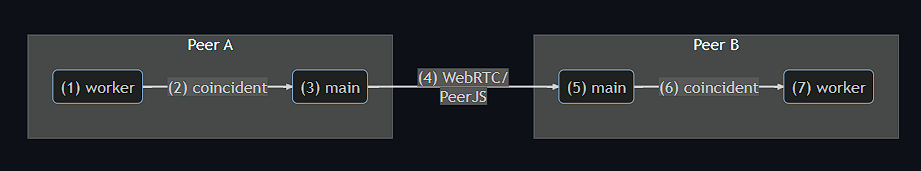
\includegraphics[width=\textwidth,height=0.9\textheight]{thesis/../figures/mpyc-web.png}
\caption{MPyC Web \label{osi-map-overlays}}
\end{figure}

\begin{enumerate}
\def\labelenumi{\arabic{enumi}.}
\item
  Python Worker on Peer A

  \begin{itemize}
  \tightlist
  \item
    creates a message that contains a secret share computed via the
    mpyc, which serializes it to binary via struct.pack(). The resulting
    message is non-ascii, but when escaped can look like this:
  \end{itemize}

\begin{Shaded}
\begin{Highlighting}[]
\StringTok{b\textquotesingle{}}\CharTok{\textbackslash{}x06\textbackslash{}x00\textbackslash{}x00\textbackslash{}x00\textbackslash{}xc9\textbackslash{}x93\textbackslash{}\textbackslash{}\textbackslash{}xc0\textbackslash{}xff\textbackslash{}xff\textbackslash{}xff\textbackslash{}xff\textbackslash{}x04\textbackslash{}x00\textbackslash{}x80\textbackslash{}x99\textbackslash{}x1b\textbackslash{}x01}\StringTok{\textquotesingle{}}
\end{Highlighting}
\end{Shaded}

  \begin{itemize}
  \tightlist
  \item
    worker calls a main thread function (sendRuntimeMessage) via a
    coincident proxy and passes the serialized value, as well as the
    destination Peer's ID (Peer B). The worker does not need to await
    the result of this call, but it does because of xworker.sync.
  \end{itemize}
\item
  Coincident handles the message by:

  \begin{itemize}
  \tightlist
  \item
    (Worker) JSON.stringify() -\textgreater{} Atomics.wait()
  \item
    (Main) JSON.parse() -\textgreater{} Run the Main Thread function
    -\textgreater{} Atomics.notify()
  \end{itemize}
\item
  Main thread on Peer A fires an event to notify PeerJS that it needs to
  transport the message and immediately returns in order to not block
  the Worker
\item
  PeerJS serializes the message with some added fields via MessagePack
  and transmits it to Peer B
\item
  Main thread on Peer B receives the message and forwards it to the
  appropriate worker callback via coincident
\item
  Coincident does the JSON.stringify() -\textgreater{} Atomics.wait()
  stuff (?) from main to worker on Peer B
\item
  Worker on Peer B handles the message by passing it to an asyncio
  coroutine that is waiting for it or stores it for later use
\end{enumerate}

\section{Implementation
details}\label{thesis__090-mpyc-web.md__implementation-details}

\section{Performance
analysis}\label{thesis__090-mpyc-web.md__performance-analysis}

\section{Security
analysis}\label{thesis__090-mpyc-web.md__security-analysis}

\subsection{Trust model}\label{thesis__090-mpyc-web.md__trust-model}

There still is a centralized service like in the Tailscale solution, but
here it is self-deployed.

\subsection{Identity}\label{thesis__090-mpyc-web.md__identity}

\section{Usability
analysis}\label{thesis__090-mpyc-web.md__usability-analysis}


\printbibliography

\end{document}
